\documentclass[usepdftitle=false]{beamer}
\directlua{pdf.setminorversion(7)}

\usetheme{Singapore}
\usefonttheme{professionalfonts}
\setbeamertemplate{navigation symbols}{}

%
% Packages
%

\usepackage{fontspec}%
\usepackage[english]{babel}%
\usepackage[babel, final]{microtype}%

\usepackage{mathtools}%
\usepackage{amsthm}%
\usepackage[ruled, longend]{algorithm2e}%
\usepackage{prftree}%
\usepackage{unicode-math}%

\usepackage{fancyvrb}%
\usepackage[newfloat]{minted}%

\usepackage{booktabs}%
\usepackage{graphicx}%
\usepackage[compatibility=false]{caption}%
\usepackage{subcaption}%

\usepackage{tikz}%
\usepackage{pgfplots}%
\usepackage{pgfplotstable}%

\usepackage[strict, autopunct]{csquotes}%
\usepackage[hyperref, citestyle=numeric-comp, backend=biber,%
maxcitenames=2, giveninits, isbn=false, url=false, doi=false]%
{biblatex}%

\usepackage{siunitx}%
\usepackage{nth}

\usepackage[shortcuts]{extdash}%

%
% Setup
%

\addbibresource{../Bibliography.bib}%
\unimathsetup{%
  math-style=ISO,%
  bold-style=ISO%
}%
\mathtoolsset{
  mathic%
}%
\graphicspath{{Figures/}{../}}%
\sisetup{%
  detect-all,%
  detect-display-math,%
  binary-units%
}%
\hypersetup{%
  unicode,
  pdfinfo={%
    Title={Author Profiling},%
    Subject={Pattern Recognition},%
    Author={Dario Gjorgjevski},%
    Keywords={Deep Learning, Neural Networks, Distributed Representations}%
  }
}%
\pgfplotsset{compat=newest}%
\usetikzlibrary{patterns, fit, positioning, calc, shapes.arrows}%

%
% Commands
%

% Notation from linear algebra
\AtBeginDocument{%
  \renewcommand*{\vec}{\symbf}%
  \newcommand*{\mat}{\symbf}%
  \newcommand*{\trans}{\top}%
}%
\DeclareMathOperator{\rank}{rank}%
\DeclareMathOperator{\lspan}{span}%
\DeclareMathOperator{\supp}{supp}%
\DeclarePairedDelimiter{\basis}{\langle}{\rangle}%
\newcommand*{\M}{\ensuremath{\mathcal{M}}}%
\newcommand*{\GL}{\ensuremath{\mathsf{GL}}}%

% Notation from probability and statistics
\DeclareMathOperator{\E}{\mathbb{E}}%
\DeclareMathOperator{\var}{var}%
\DeclareMathOperator{\cov}{cov}%

%
% Title
%

\title{Author Profiling}%
\subtitle{Using Deep Learning to Identify Age Groups and Genders}%
\author[Dario Gj.]{%
  Dario Gjorgjevski\\%
  \href{mailto:gjorgjevski.dario@students.finki.ukim.mk}%
  {\nolinkurl{gjorgjevski.dario@students.finki.ukim.mk}}%
}%
\institute[FCSE]{%
  Faculty of Computer Science and Engineering\\%
  Ss.\ Cyril and Methodius University in Skopje%
}%
\date{November 4, 2017}

%
% Logo
%

%\logo{
\includegraphics[height=0.66cm]{Logo_ФИНКИ.pdf}}

%
% Table of contents
%

\AtBeginSection{%
  \begin{frame}{Contents}
    \tableofcontents[currentsection]
  \end{frame}%
}

%
% Document
%

\begin{document}

\begin{frame}[plain, noframenumbering]
  \titlepage%
\end{frame}

\section{Introduction}

\begin{frame}{Motivation}
  \begin{itemize}
  \item Huge volume of user\-/generated content \(\implies\) appealing
    to profile users based on it.
  \item Profiling has multi\-/faceted advantages:
    \begin{description}
    \item[Commercial] Analyze the demographics of people that like or
      dislike certain products.
    \item[Forensic] Find out the linguistic profile of the author of a
      harassing text message and identify certain characteristics
      (\emph{language as evidence}).
    \end{description}
  \end{itemize}
\end{frame}

\begin{frame}{Task}
  \begin{definition}[Author Profiling]
    Author profiling is the task of identifying certain features of
    authors of text.
  \end{definition}
  \begin{itemize}
  \item We will focus on the \emph{genders} and \emph{age groups} of
    authors of Twitter posts.
  \item Genders are either \Verb+male+ or \Verb+female+.
  \item Age groups are \num{18}\==\num{24}, \num{25}\==\num{34},
    \num{35}\==\num{49}, \num{50}\==\num{64}, and
    \num{65}\==\Verb+xx+.
  \end{itemize}
\end{frame}

\begin{frame}{Dataset}
  \begin{itemize}
  \item Data are provided as part of the PAN 2016 event\footnotemark.
  \item There are \num{277792} tweets written in English by \num{436}
    users, or an average of \num{637.14} tweets per user.
  \item \num{218} users are male and \num{218} are female.
  \item The distribution of age groups is given in
    table~\autoref{tab:age-groups}.
  \item We additionally used the data provided by the 2013, 2014, and
    2017 PAN events for the unsupervised part of our classification
    pipeline (\structure{stay tuned}).
  \end{itemize}
  \footnotetext[1]{\url{http://pan.webis.de/clef16/pan16-web/author-profiling.html}}
\end{frame}

\begin{frame}{Age Groups}
  \begin{table}
    \centering
    \caption{Distribution of age groups.}\label{tab:age-groups}
    \begin{tabular}{c S[table-format=3]}
      \toprule
      Age group & {Number of users} \\
      \midrule
      \num{18}\==\num{24} & 28 \\
      \num{25}\==\num{34} & 140 \\
      \num{35}\==\num{49} & 182 \\
      \num{50}\==\num{64} & 80 \\
      \num{64}\==\Verb+xx+ & 6 \\      
      \bottomrule
    \end{tabular}
  \end{table}
  One can see that there is \alert{class imbalance} here.  However, we
  are \alert{not} going to attempt to rectify this by weighing or
  resampling.
\end{frame}

\section{Preprocessing}

\begin{frame}[fragile]{Parsing}
  \begin{itemize}
  \item Data are given in XML files: there is one XML file per author
    named by the author's hexadecimal ID\@.
  \item We used the Beautiful Soup library to parse the files.
  \item Additionally, there is a file called \Verb+truth.txt+ which
    consists of lines of the form
    \begin{Verbatim}
    <filename>:::<gender>:::<age-group>
    \end{Verbatim}
    and gives the ground truth.
  \end{itemize}
\end{frame}

\begin{frame}{Normalization}
  \begin{enumerate}
  \item Hash tags, replies, and external links are replaced by new and
    unique tokens.
  \item Tweets are tokenized into words using the Punkt
    tokenizer~\autocite{KS06} from NLTK, the natural language toolkit.
  \item Abbreviations and nonstandard words such as \enquote{ur} and
    \enquote{lol} are converted to their standard forms using a
    dictionary constructed from the ACL 2015 workshop on noisy
    user\-/generated content~\autocite{HCB12}.
  \end{enumerate}
\end{frame}

\section{Classification Pipeline}

\begin{frame}{Distributed Representations}{Motivation}
  The \textsf{Doc2Vec} model learns distributed representations of
  both words and entire documents.  In our case,
  \(\mathrm{document} \coloneqq \mathrm{author}\).
  \begin{itemize}
  \item Semantically related entities, e.g., Prague, Rome, Berlin,
    etc., should be close to each other.
  \item Two entities are considered close if they appear in the same
    context (\textsf{Word2Vec}~\autocite{Mik13}).
  \item The context is a simple window of \(k\) words to the left and
    to the right of a target word.
  \item The \enquote{leftovers} of the context are explained by the
    \emph{document's ID} itself (\textsf{Doc2Vec}~\autocite{LM14}).
  \end{itemize}
\end{frame}

\begin{frame}{Distributed Representations}{Architecture}
  \begin{figure}
    \centering
    \begin{subfigure}[b]{.15\textwidth}
      \mbox{}
    \end{subfigure}
    \begin{subfigure}[b]{.40\textwidth}
      \centering
      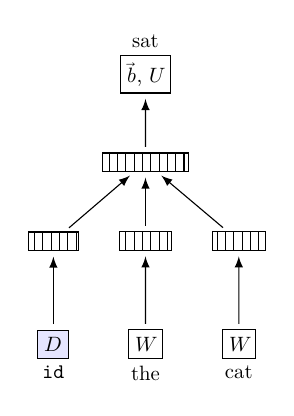
\begin{tikzpicture}[>=latex, shorten >=2pt, shorten <=2pt, scale=.75, every node/.style={transform shape}]
        \node[draw, rectangle, label=below:\Verb+id+, fill=blue!10] (doc) {\(\mat D\)};%
        \node[draw, rectangle, right=of doc, label=below:the] (the) {\(\mat W\)};%
        \node[draw, rectangle, right=of the, label=below:cat] (cat) {\(\mat W\)};%

        \node[draw, rectangle, fit=(doc.west) (doc.east), pattern=vertical lines, above=of doc] (in_doc) {};%
        \node[draw, rectangle, fit=(the.west) (the.east), pattern=vertical lines, above=of the] (in_the) {};%
        \node[draw, rectangle, fit=(cat.west) (cat.east), pattern=vertical lines, above=of cat] (in_cat) {};%

        \node[draw, rectangle, fit={($(the.west) + (-8pt,0pt)$) ($(the.east) + (8pt,0pt)$)}, pattern=vertical lines, above=2cm of the] (in) {};%
        \node[draw, rectangle, above=of in, label=above:sat] (out) {\(\vec b\), \(\mat U\)};%
      
        \foreach \word in {doc, the, cat}{%
          \draw[->] (\word) -- (in_\word);%
          \draw[->] (in_\word) -- (in);%
        }%
        \draw[->] (in) -- (out);%

        \useasboundingbox (current bounding box);%
        \node[left=of doc, outer sep=0] (embed) {embed};%
        \node[above=2cm of embed, outer sep=0] (concatenate) {concatenate};%
        \node[above=1cm of concatenate, outer sep=0] {softmax};%
      \end{tikzpicture}
      \caption{DM model.}\label{fig:dm}
    \end{subfigure}
    \begin{subfigure}[b]{.40\textwidth}
      \centering
      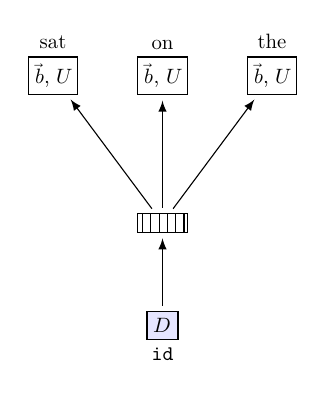
\begin{tikzpicture}[>=latex, shorten >=2pt, shorten <=2pt, scale=.75, every node/.style={transform shape}]
        \node[draw, rectangle, label=below:\Verb+id+, fill=blue!10] (doc) {\(\mat D\)};%
        \node[draw, rectangle, fit=(doc.west) (doc.east), pattern=vertical lines, above=of doc] (in) {};%
        \node[draw, rectangle, above=2cmof in, label=above:on] (on) {\(\vec b\), \(\mat U\)};%
        \node[draw, rectangle, left=of on, label=above:sat] (sat) {\(\vec b\), \(\mat U\)};%
        \node[draw, rectangle, right=of on, label=above:the] (the) {\(\vec b\), \(\mat U\)};%

        \draw[->] (doc) -- (in);%
        \foreach \word in {sat, on, the}{%
          \draw[->] (in) -- (\word);%
        }%
      \end{tikzpicture}
      \caption{DBOW model.}\label{fig:dbow}
    \end{subfigure}
    \caption{\textsf{Doc2Vec} with embeddings \(\mat W\) and \(\mat D\).}
  \end{figure}
\end{frame}

\begin{frame}{Distributed Representations}{Learning}
  \begin{itemize}
  \item We trained the DM model (figure~\autoref{fig:dm}) using
    Gensim~\autocite{RS12} on \num{1047358} posts from social media
    (PAN 2013, 2014, and 2017) to learn embeddings of size \num{256}.
  \item Training was carried for \num{20} epochs using a context
    window of size \num{8}.
  \item Some examples for closest representations can be seen on
    figure~\autoref{fig:examples}.
  \end{itemize}
\end{frame}

\begin{frame}[fragile]{Distributed Representations}{Examples}%
  \begin{figure}
    \begin{columns}
      \begin{column}{.5\textwidth}
\begin{minted}[fontsize=\footnotesize]{python}
>>> mdl.most_similar('substantial')

[('higher', 0.72),
 ('large', 0.70),
 ('high', 0.69),
 ('significant', 0.6),
 ('huge', 0.6),
 ('reduced', 0.6),
 ('massive', 0.59),
 ('increased', 0.58),
 ('considerable', 0.57),
 ('enormous', 0.56)]
\end{minted}
      \end{column}%
      \begin{column}{.5\textwidth}
\begin{minted}[fontsize=\footnotesize]{python}
>>> mdl.most_similar('trump')

[('ivanka', 0.5),
 ('donald', 0.41),
 ('gould', 0.4),
 ('melania', 0.38),
 ('selby', 0.38),
 ('osullivan', 0.35),
 ('finalist', 0.34),
 ('hudson', 0.31),
 ('qingyang', 0.31),
 ('ferguson', 0.31)]
\end{minted}
      \end{column}
    \end{columns}
    \caption{Similarities between the learned word
      vectors.}\label{fig:examples}
  \end{figure}
\end{frame}

\begin{frame}{The Pipeline}
  \begin{enumerate}
  \item Words are padded to a length of \num{512}, transformed to
    their distributed representations, and fed to two CNNs:
    \begin{enumerate}
    \item \num{128} filters using a kernel size of \num{4}, rectified
      linear units (ReLUs) for activation, and max\=/pooled with a
      factor of \num{4}; and
    \item \num{128} filters using a kernel size of \num{4}, ReLUs for
      activation, and max\=/pooled with a factor of \num{16}.
    \end{enumerate}
  \item Author IDs are transformed to their distributed
    representations and fed to a densely\-/connected network of
    \num{128} ReLUs.
  \item The two outputs are concatenated and fed to:
    \begin{enumerate}
    \item Densely\-/connected layer of \num{128} ReLUs;
    \item Densely\-/connected layer of \num{32} ReLUs; and a
    \item Softmax panel for classification.
    \end{enumerate}
  \end{enumerate}
\end{frame}

\section{Results and Future Work}

\begin{frame}{Results}
  \begin{itemize}
  \item Training the architecture for \num{3} epochs yielded an
    accuracy of \SI[round-mode=places,
    round-precision=2]{81.300892040779427}{\percent} for gender, and
    \SI[round-mode=places, round-precision=2]{61.18}{\percent} for age
    groups.
  \item The accuracy was estimated using \num{1/3} of the data for
    validation.
  \item Better results than the ones observed at PAN 2016.
  \end{itemize}
\end{frame}

\begin{frame}{Future Work}
  \begin{itemize}
  \item We would like to determine why over\-/fitting began to occur
    after the \nth{3} epoch.  It might be worthwhile to apply \(L_1\)
    or \(L_2\) regularization, or more aggressive dropout.
  \item Lexical normalization is not perfect: since a dictionary is
    used, \enquote{ur} will always be translated to \enquote{your}
    even though it might sometimes stand for \enquote{you are}.
  \item An obvious improvement is to train the distributed
    representations on more data, and perhaps lemmatize the texts
    before processing them.
  \end{itemize}
\end{frame}

\begin{frame}[allowframebreaks]{References}
  \printbibliography[heading=none]
\end{frame}

\end{document}

%%% Local Variables:
%%% mode: latex
%%% TeX-command-extra-options: "-shell-escape"
%%% TeX-engine: luatex
%%% TeX-master: t
%%% End: